\documentclass[11pt,a4paper]{article}

% EventIQ technical report. Compiles on Overleaf with pdfLaTeX out of the box.
\usepackage[utf8]{inputenc}
\usepackage[T1]{fontenc}
\usepackage{lmodern}
\usepackage{microtype}
\usepackage[margin=1in]{geometry}
\usepackage{booktabs}
\usepackage{array}
\usepackage{xcolor}
\usepackage{listings}
\usepackage{enumitem}
\usepackage{titlesec}
\usepackage{caption}
\usepackage{graphicx}
\usepackage[hidelinks]{hyperref}
\usepackage{fancyhdr}

\pagestyle{fancy}
\fancyhf{}
\fancyhead[L]{\small\scshape EventIQ}
\fancyhead[R]{\small Network security log analysis}
\fancyfoot[C]{\thepage}
\renewcommand{\headrulewidth}{0.3pt}
\renewcommand{\footrulewidth}{0pt}

\definecolor{ink}{HTML}{1B1F24}
\definecolor{accent}{HTML}{2F5AA8}
\definecolor{soft}{HTML}{5B6470}
\definecolor{codebg}{HTML}{F4F5F7}

\titleformat{\section}{\normalfont\Large\bfseries\color{ink}}{\thesection}{0.6em}{}
\titleformat{\subsection}{\normalfont\large\bfseries\color{ink}}{\thesubsection}{0.6em}{}
\setlist{itemsep=2pt,topsep=3pt}
\setlength{\emergencystretch}{3em}

\lstset{
  basicstyle=\ttfamily\small,
  backgroundcolor=\color{codebg},
  frame=single, rulecolor=\color{codebg},
  breaklines=true, columns=fullflexible,
  xleftmargin=8pt, xrightmargin=8pt, aboveskip=8pt, belowskip=8pt,
}

\newcommand{\code}[1]{\texttt{#1}}

\title{\vspace{-1.2cm}\textbf{EventIQ}\\[2pt]
\large Detecting distributed attacks in a million log rows,\\and measuring how well}
\author{Muhammad Ismail \\ \small SOC Internship Project, Ebryx (blue team)}
\date{July 2026}

\begin{document}
\maketitle
\vspace{-0.4cm}

\begin{abstract}
\noindent
EventIQ is a Python tool that analyses a 1,000,000-row network and
authentication log, identifies the attacks inside it, ranks them by risk, and
produces a report, a dashboard, and deployable Wazuh and Sigma rules. Its design
turns on one decision: the dataset ships with a label column that names the
attacks, and the detection engine never reads it. Detection works from raw fields
only; the label is held out and used solely to score precision, recall and F1.
On the provided file the five detected campaigns score 1.000 on all three
metrics, while a naive ``any failed login'' baseline scores 0.463 precision. The
report also names two detections that this data cannot support and shows the
numbers that make them traps. This document explains the data, the method, the
validation, and the limitations.
\end{abstract}

\vspace{-0.3cm}
{\small\tableofcontents}
\vspace{0.3cm}

\begin{figure}[h]
\centering
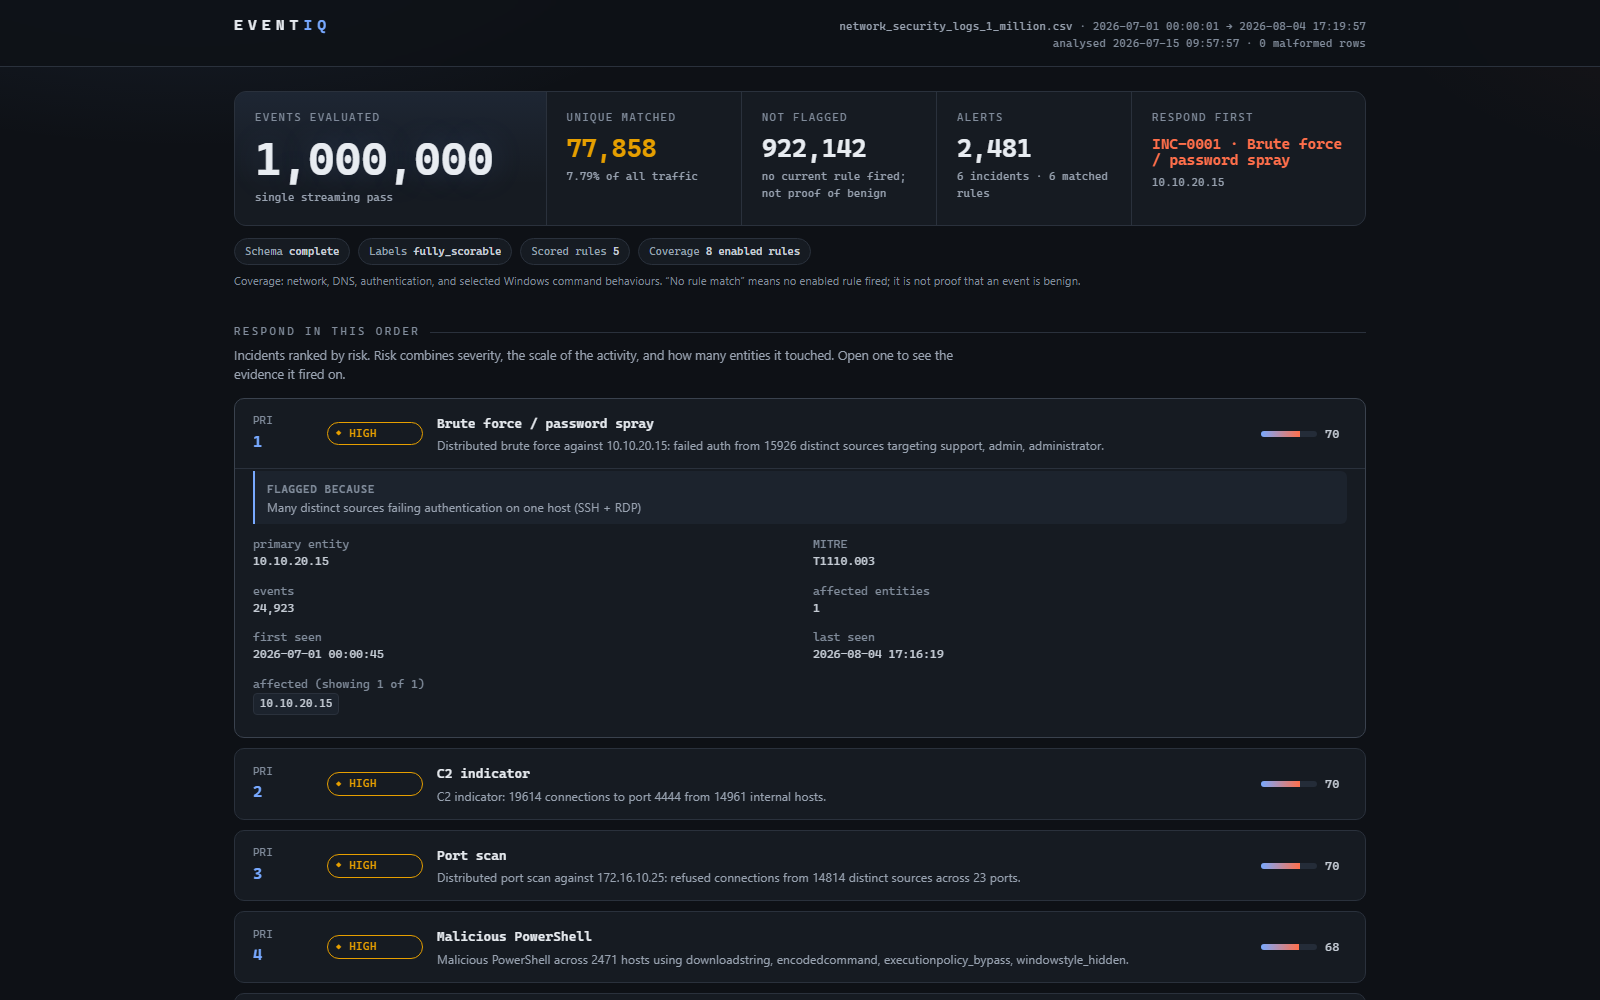
\includegraphics[width=\textwidth]{figures/dashboard-overview.png}
\caption{The dashboard after analysing the full 1,000,000-row file: 2,481 alerts collapsed into 6 ranked incidents, with the top incident's evidence already expanded.}
\end{figure}

\section{Problem}

A security team has a log file with a million lines of network connections,
authentication attempts, DNS activity and system events. Somewhere inside are
real attacks mixed with normal traffic. Reading it by hand is not possible. The
tempting shortcut, trusting the file's own labels, proves nothing about whether
the tool can actually detect.

The assignment measures four things at once: Python engineering, networking
fundamentals, log-analysis method, and security-investigation reasoning. The
interesting part is not writing a rule that matches a label. It is detecting an
attack that has been deliberately shaped to defeat the obvious rule, and then
proving the detection is accurate rather than asserting it.

\section{The dataset}

The input is one CSV, 132\,MB, 1,000,000 rows, sixteen columns, spanning
2026-07-01 to 2026-08-04 (35 days). Every figure in this section came from
profiling the file directly, not from assumption.

\begin{table}[h]
\centering
\small
\begin{tabular}{@{}lr@{\hspace{2em}}lr@{}}
\toprule
Event type & Rows & Event type & Rows \\
\midrule
NETWORK\_CONNECTION & 560,694 & FAILED\_LOGIN\_BURST & 24,923 \\
DNS\_QUERY & 159,342 & PORT\_SCAN & 16,842 \\
LOGIN & 120,383 & SUSPICIOUS\_DNS & 10,176 \\
FILE\_ACCESS & 59,581 & DNS\_TUNNELING & 5,044 \\
POWERSHELL & 40,088 & SUSPICIOUS\_POWERSHELL & 2,927 \\
\bottomrule
\end{tabular}
\caption{Distribution of the held-out \code{event\_type} label.}
\label{tab:event-types}
\end{table}

\subsection{The data ships with its own answer key}

The \code{event\_type} and \code{severity} columns are labels, not observations.
A tool that filters \code{event\_type == "PORT\_SCAN"} and calls that detection
has detected nothing. It has read the answer key. This drives the central design
decision of the project:

\begin{quote}
The detection engine reads only raw observable fields: timestamp, IPs, ports,
protocol, service, username, status, domain, command, bytes. It never reads
\code{event\_type} or \code{severity}. Those two columns are held out and used
only to score the detectors.
\end{quote}

That gives the project something most submissions of this kind do not have: a
measured precision, recall and F1 per rule, against ground truth.

\subsection{The attacks are distributed, which breaks the textbook rules}

\textbf{Port scan.} 16,842 events, but from 14,814 distinct source IPs, 87\,\% of
which appear exactly once hitting exactly one port. Every source sits in
\code{203.0.0.0/16} and every one targets the single host \code{172.16.10.25}.
All are blocked, with \code{bytes\_received} of 0.

\textbf{Brute force.} 24,923 events from 15,926 distinct source IPs in
\code{185.199.0.0/16}, all onto \code{10.10.20.15}, split across SSH (port 22,
12,400 events) and RDP (port 3389, 12,523 events), all failed, concentrated on
the usernames \code{support}, \code{admin} and \code{administrator}.

The classic rule ``alert when one source IP contacts more than $N$ ports in a
minute'' fires zero times here. Worse, the timestamps are uniform across all 35
days at roughly 4\,\% of events per hour, so a five-minute sliding window
accumulates about two events and never crosses a distinct-source threshold. The
signal is convergent, so the detector must be too: it pivots on the
\emph{destination} and counts how many distinct sources and subnets converge on
it over the whole batch. Benign traffic to the scan target was 6 events in 35
days; to the brute-force target, 2. A destination-pivot detector is nearly
noise-free here.

\subsection{The noise floor}

28,889 \code{LOGIN} rows carry a \code{FAILED} status but are not part of the
burst. They are ordinary background authentication failures. A detector that
alerts on ``any failed login'' gets high recall and terrible precision.
Separating the real distributed campaign from this background is the actual
detection problem, and it is what makes the precision number meaningful rather
than a row of ones by construction.

\section{Detection method}

Six detectors read the stream (Table~\ref{tab:detectors}). Each keys on
structure, never on a specific address, so nothing about this file is
hardcoded. Thresholds live in \code{config/default.yml} and every one traces
to a primary source recorded in \code{docs/RESEARCH.md}.

\begin{table}[h]
\centering
\small
\renewcommand{\arraystretch}{1.25}
\begin{tabular}{@{}p{2.9cm}p{6.9cm}p{2.6cm}@{}}
\toprule
Detector & Fires when & MITRE \\
\midrule
port\_scan & Many distinct sources refused by one host, across many ports & T1046 \\
brute\_force & Many distinct sources failing auth on one host (SSH/RDP) & T1110.003 \\
dns\_tunnel & A parent domain with high-entropy, long, and numerous subdomains & T1071.004 \\
suspicious\_domain & Domain on the indicator list or a flagged TLD & T1071.004 \\
powershell & Encoded / download-cradle / hidden / bypass pattern in the command & T1059.001 \\
c2\_port & Traffic to a known handler port (4444) & T1571 \\
\bottomrule
\end{tabular}
\caption{The six detectors. Techniques are keyed by ID, since MITRE renamed
several tactics and Wazuh and Sigma still emit the old strings.}
\label{tab:detectors}
\end{table}

\begin{figure}[h]
\centering
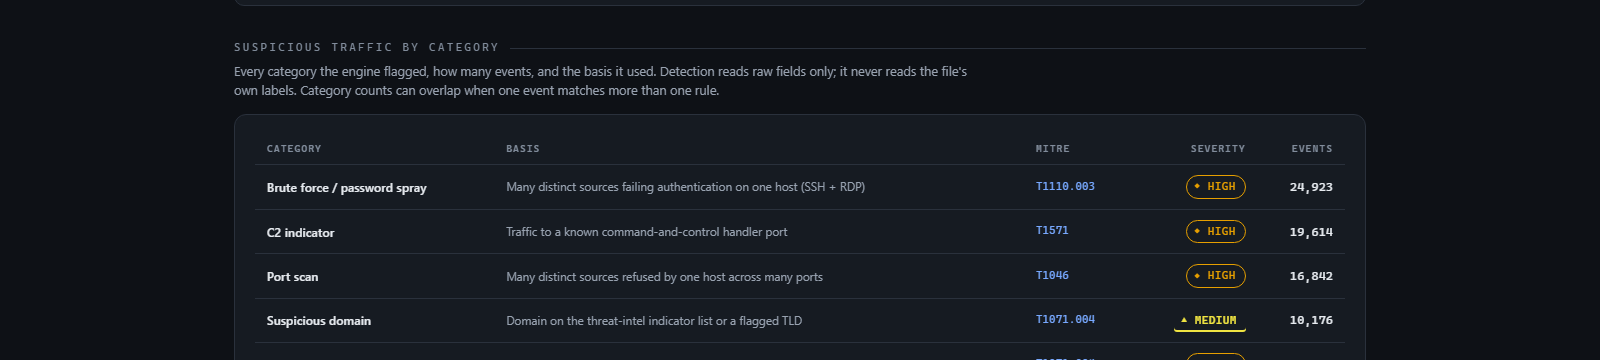
\includegraphics[width=\textwidth]{figures/dashboard-categories.png}
\caption{Every category the engine flagged, the raw-field basis it used, and the observed MITRE technique. This table is generated straight from the JSON report, not written by hand.}
\end{figure}

\subsection{The distributed detectors}

Both the scan and the brute force use the same primitive: a per-destination
accumulator that counts distinct sources, distinct \code{/24} subnets, and
distinct ports over the pass. The port-scan detector only tracks refused
connection attempts, which is both the scan signature and the reason its memory
stays bounded to the handful of hosts that receive refused traffic rather than
every destination in the file. The thresholds were calibrated against the
observed benign ceiling:

\begin{itemize}
\item Brute force: the busiest benign host had 28 distinct failing sources; the
campaign had 15,926. The threshold sits at 50, a wide margin either way.
\item Port scan: the busiest benign host had 758 sources but zero refused and one
service port; the scan target had 14,814 sources, all refused, across 23 ports.
\end{itemize}

\subsection{The content detectors}

\textbf{DNS tunneling} combines three signals, because entropy alone
false-positives on legitimate high-entropy names. A parent domain fires only when
it carries subdomains that are simultaneously high-entropy (Shannon entropy above
3.0 on the longest label), long (label length at least 20), and numerous (at
least five unique subdomains). The tunneling channel in this file used
54-character random labels under one parent with 5,044 unique subdomains, against
only ten benign domains in the entire file.

\textbf{Suspicious domains} match an indicator list plus a conservative bad-TLD
net. Indicator lists in configuration are not hardcoded constants in the sense
that matters; they are threat intelligence fed to a rule, which is exactly how a
SOC operates.

\textbf{Malicious PowerShell} matches four command families: encoded command,
download cradle, hidden window, and execution-policy bypass. It groups by source
host, so the finding is per compromised endpoint.

\textbf{C2 indicator} flags traffic to a known handler port and rolls all of it
into one finding with the internal hosts and external destinations ranked, rather
than emitting one alert per destination.

\section{Risk scoring and incident correlation}

Row-level alerts are accurate but not directly usable: the file produces 2,481 of
them. A risk layer assigns each alert points from its severity band and the
magnitude of what it saw, sums them per entity, and adds a bonus when more than
one detector implicates the same entity, which is the core idea of risk-based
alerting. A correlation layer then groups alerts into incidents by campaign,
names the primary entity, and writes a plain-English narrative. The result is
\textbf{six ranked incidents}, each expandable to its evidence and affected
entities. Incident risk also factors campaign breadth, so a PowerShell campaign
across 2,471 hosts outranks a scan against a single host.

\section{Validation}

Validation is the point of the held-out labels. It is the only place
\code{event\_type} is read, and it is the scorer, never a detector. Results are
in Table~\ref{tab:results}.

\subsection{The match rule}

Each fired alert records the exact source-row identifiers it fired on. A row is
flagged by rule $R$ if its identifier is in the union of those sets for $R$'s
alerts. For rule $R$ with campaign label $L$:

\begin{itemize}
\item flagged and label $=L$: true positive
\item flagged and label $\neq L$: false positive
\item not flagged and label $=L$: false negative
\end{itemize}

Event-level scoring is used rather than an entity plus time-window rule because a
host-entity detector like PowerShell must be judged on the command events it
flagged, not on all the benign traffic those hosts also generate. An earlier
entity-window rule gave PowerShell a false precision of 0.034 for exactly that
reason; event-level scoring corrected it to 1.000.

\subsection{Results}

\begin{table}[h]
\centering
\small
\begin{tabular}{@{}lrrrrrr@{}}
\toprule
Rule & Precision & Recall & F1 & TP & FP & FN \\
\midrule
brute\_force & 1.000 & 1.000 & 1.000 & 24,923 & 0 & 0 \\
port\_scan & 1.000 & 1.000 & 1.000 & 16,842 & 0 & 0 \\
dns\_tunnel & 1.000 & 1.000 & 1.000 & 5,044 & 0 & 0 \\
suspicious\_domain & 1.000 & 1.000 & 1.000 & 10,176 & 0 & 0 \\
powershell & 1.000 & 1.000 & 1.000 & 2,927 & 0 & 0 \\
\midrule
\textbf{Overall} & \textbf{1.000} & \textbf{1.000} & \textbf{1.000} & \textbf{59,912} & \textbf{0} & \textbf{0} \\
\bottomrule
\end{tabular}
\caption{Scored against held-out labels on the full file.}
\label{tab:results}
\end{table}

The comparison that gives these numbers meaning: a naive ``any failed login''
rule would flag 53,812 rows to catch the 24,923 real burst rows, a precision of
0.463. The distributed detector reaches the same recall without that cost.

\begin{figure}[h]
\centering
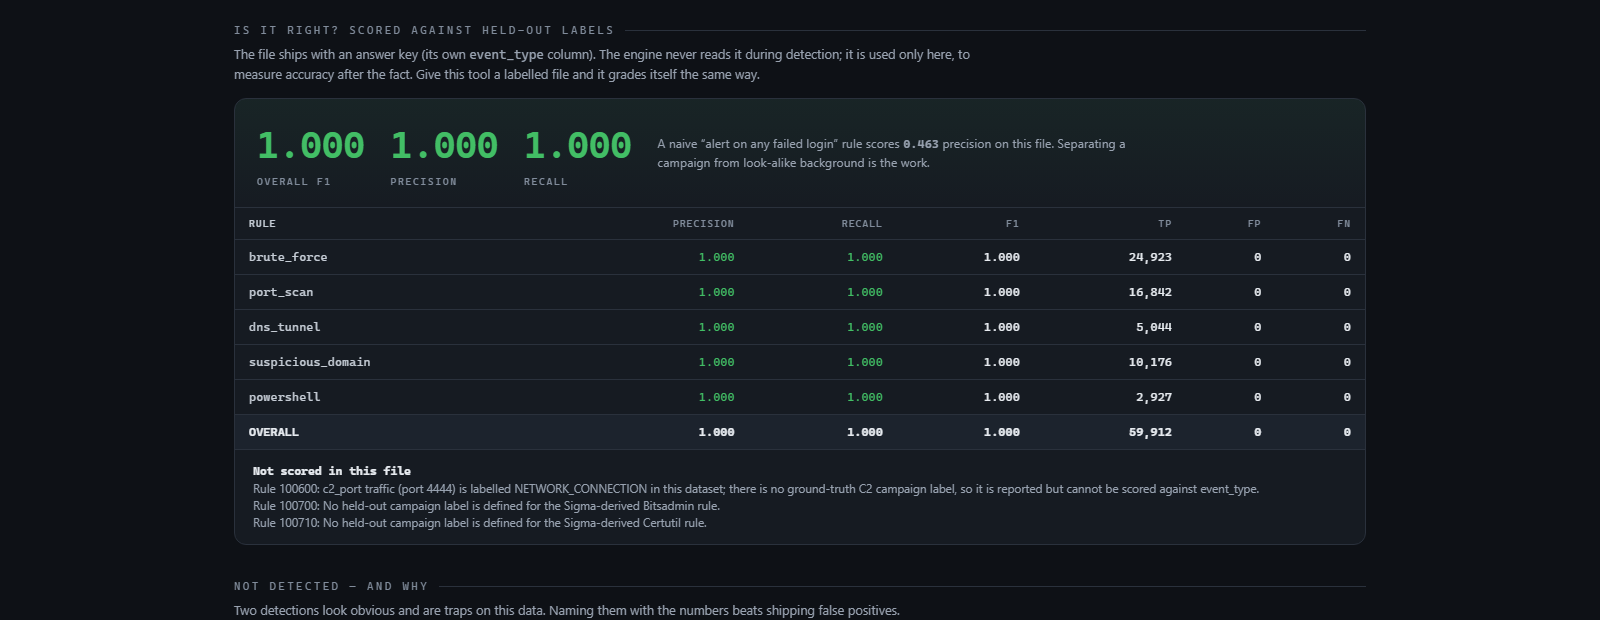
\includegraphics[width=\textwidth]{figures/dashboard-validation.png}
\caption{The same scoring table rendered live in the dashboard, computed from the held-out \code{event\_type} column after detection finishes.}
\end{figure}

\subsection{The C2 finding is reported but not scored}

The port-4444 traffic has no ground-truth label. Of its 19,614 events, 17,946 are
labelled \code{NETWORK\_CONNECTION}, 978 \code{SUSPICIOUS\_POWERSHELL} and 690
\code{PORT\_SCAN}. There is no C2 campaign label, so scoring it against
\code{event\_type} would be misleading. It is reported as an indicator-based
detection and left out of the score, and the tool says so.

\section{Two detections this data cannot support}

Both are on every network-log tutorial. Both would be pure false positives here.

\textbf{Exfiltration by byte volume.} The byte columns are uniform noise. The
median total is about 3.5\,MB for every event type, including DNS queries. A
volume rule would rank random benign rows as the top exfiltration events.

\textbf{Off-hours activity and beaconing.} Timestamps are uniform at about 4\,\%
of events per hour, 24 hours a day, with no periodic interval. There is no
business-hours baseline and no beacon to recover.

Naming these with the numbers is a stronger signal than adding two rules that
quietly produce garbage. Both appear in the report's \code{not\_detected}
section.

\section{Architecture and performance}

\begin{lstlisting}
CSV -> streaming reader (drops event_type/severity) -> Event
    -> AnalysisEngine (single pass, six detectors)
    -> Alerts -> risk scoring + incident correlation
    -> JSON report -> HTML dashboard | Wazuh XML | Sigma YAML
    -> validate (separate pass, reads held-out labels, scores)
\end{lstlisting}

The engine is pure standard library on the hot path, with \code{jinja2} and
\code{pyyaml} only for rendering and configuration. It streams the file in a
single pass, so peak memory is a function of active-entity count rather than file
size. The full 1,000,000-row file analyses in about 45 seconds with peak memory
under 150\,MB. An early version reached 1,082\,MB by building a state object for
every one of about 423,000 destinations; restricting the scan detector to refused
connections dropped that to 75\,MB.

The ``never reads the label'' guarantee is mechanical, not a promise. The
\code{Event} object has no \code{event\_type} or \code{severity} field, and a
test scans the detector sources and fails the build if either string appears.

\subsection{Scaling}

Distinct-source counting is exact here and fits comfortably, because there are
tens of thousands of active entities rather than billions. The distinct sets are
the seam where a HyperLogLog sketch would go at 100 times the scale, trading a
little accuracy in the evidence counts for constant memory. That is a deliberate
non-goal for this dataset rather than an oversight.

\section{Speaking the team's language: Wazuh and Sigma}

EventIQ exports the detections as deployable rules. The distributed detectors
become Wazuh frequency rules that count different source IPs against the same
destination, and Sigma \code{value\_count} correlation rules, since there is no
stock Sigma rule for a distributed campaign and Wazuh's \code{0095} SSH rule is
the reference for the shape. The content detectors become field and regular
expression matches. Rule identifiers sit in the custom 100000--120000 band, and
levels come from configuration. Where a static rule cannot reproduce the Python,
DNS-tunneling entropy is the clear case, the export says so and provides a coarse
long-random-label net instead. Deploying these needs a decoder mapping this CSV's
columns onto the standard fields, which is the team's step and out of scope here.

\section{Limitations and future work}

\begin{itemize}
\item The perfect scores reflect a synthetic dataset with clean campaigns.
Real traffic would not separate this cleanly, and the thresholds would need
retuning against a real baseline. The method transfers; the numbers would not.
\item Detection is batch over one CSV schema. A streaming deployment would move
the destination accumulators behind a time-bucketed window and, at large scale,
behind a distinct-count sketch.
\item The optional narrative and live-server layers were scoped as could-haves
and left off by default; deterministic rules do all of the detecting.
\end{itemize}

\section{Conclusion}

The result that matters is not the 1.000 F1 on its own; a rule that reads the
label would also score 1.000 and mean nothing. It is that the engine reached
those numbers without ever seeing the label, separated a distributed campaign
from tens of thousands of look-alike background events, and was honest about the
two things the data could not support. That is the difference between matching an
answer key and doing detection.

\section*{Reproducing these results}

Every number in this report comes from running the tool directly against the
supplied file, not from a cached artifact:

\begin{lstlisting}
python -m venv .venv && . .venv/Scripts/activate
pip install -e ".[dev]"

eventiq analyze network_security_logs_1_million.csv \
    -o report.json --jsonl alerts.jsonl --html dashboard.html --validate

eventiq validate network_security_logs_1_million.csv
eventiq export --wazuh eventiq_wazuh_rules.xml --sigma eventiq_sigma.yml
\end{lstlisting}

\code{pytest -q}, \code{ruff check .} and \code{mypy src} all pass. The
no-label-leak guard test fails the build on its own if a detector source file
so much as mentions \code{event\_type}.

\section*{Sources}

Thresholds and platform claims are sourced in \code{docs/RESEARCH.md} against
official documentation only. Primary references: MITRE ATT\&CK technique pages
(\href{https://attack.mitre.org}{attack.mitre.org}) for T1046, T1110.003,
T1071.004, T1059.001 and T1571; the Wazuh documentation
(\href{https://documentation.wazuh.com}{documentation.wazuh.com}) for rule levels
and the \code{0095} SSH ruleset; and SigmaHQ
(\href{https://github.com/SigmaHQ/sigma}{github.com/SigmaHQ/sigma}) for the
correlation-rule format.

\end{document}
